\documentclass{article}
\usepackage{tipa}
\usepackage{graphicx, cleveref}

\title{Audio Analysis}
\author{   
	Clarence Ang,
	Clive Ang,
	Roan Campo,
	Zhean Ganituen
}
\begin{document}
	\maketitle
	
	\section{Pronunciation of ``Halo-Halo''}
	
	The Filipino dessert \emph{Halo-Halo} is often mispronounced, largely due to
	differences between Tagalog and English orthography. The name is also
	frequently confused with the common Tagalog expression \emph{halo-halo}
	(``mixed together'').\footnote{English translation: \emph{mixed together}. For
		example, ``\emph{Pinag-halo-halo ang mga estudyante sa iba't ibang seksyon}'':
		``The students were \emph{mixed together} into different sections''.}
	
	The literal pronunciation of the Filipino word ``halo-halo'' is a reduplication
	of the lexeme ``halo'' as /\textipa{halo}/ or /\textipa{hal'o}/, with a glottal
	stop occurring between the alveolar lateral approximant /\textipa{l}/ and the
	close-mid back rounded vowel /\textipa{o}/. Another variant is the
	reduplication of the phoneme ``halu'' as /\textipa{halu}/ or /\textipa{hal'u}/.
	
	We discussed the variations of the pronunciations of \emph{Halo-Halo} and
	\emph{halo-halo} and their analysis using PRAAT.
	
	For brevity, we will use ``\emph{Halo-Halo}'' to refer to the dessert, and
	``\emph{halo-halo}'' to refer to the adjectival or verbal expression.
	
	\subsection{Mispronunciations of ``Halo-Halo''}
	
	Figure~\ref{fig:halo} illustrates the spectrogram corresponding to each
	mispronunciation of ``Halo-Halo''.
	
	\paragraph{Reduplication of /\textipa{halo}/} The spectrogram in
	\Cref{fig:halo} shows a continuous and repeating speech pattern.
	
	\begin{figure}
		\centering
		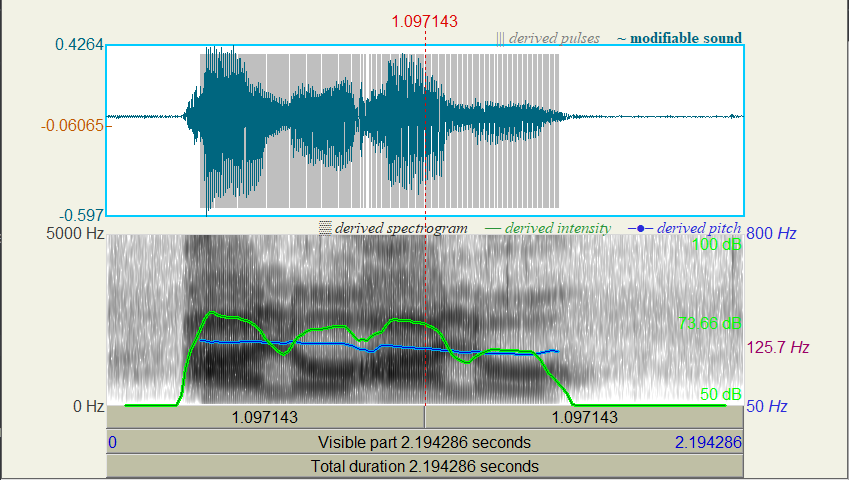
\includegraphics[width=0.65\linewidth]{img/halo.png}
		\caption{Reduplication of /\textipa{halo}/}\label{fig:halo}
	\end{figure}
	
	\paragraph{Reduplication of /\textipa{hal'o}/} \Cref{fig:hal'o} shows repetitive speech pattern with
	an abrupt stop in between each root word due to the glottal stop /\textipa{l'o}/. In fact, this is the
	correct pronunciation of ``halo-halo''.
	
	\begin{figure}
		\centering
		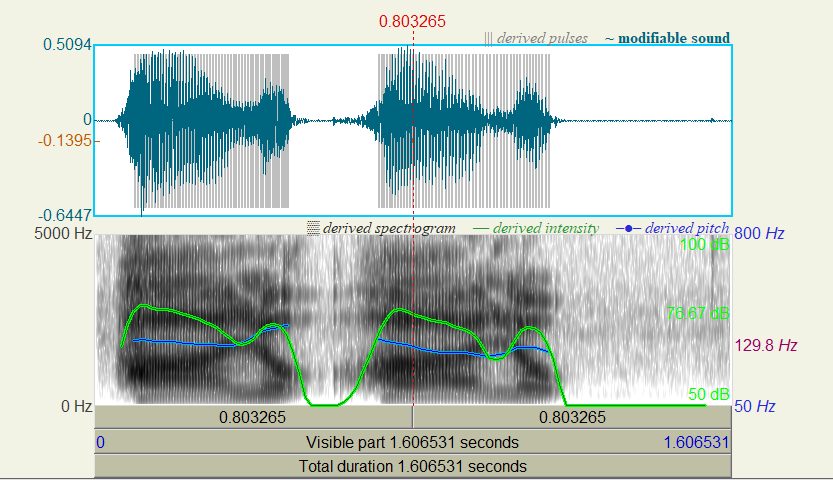
\includegraphics[width=0.65\linewidth]{img/hal_o.png}
		\caption{Reduplication of /\textipa{hal'o}/}\label{fig:hal'o}
	\end{figure}
	
	\paragraph{Reduplication of /\textipa{halu}/} \Cref{fig:halu} shows continuous and repeating
	speech pattern.
	
	\begin{figure}
		\centering
		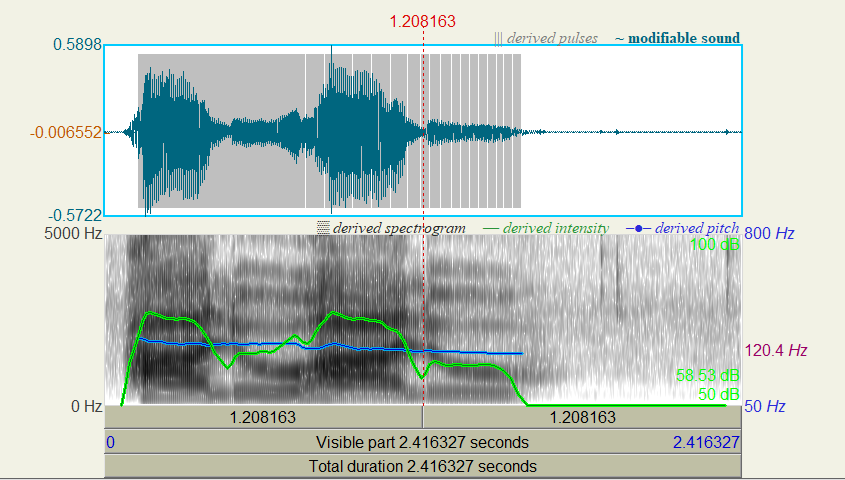
\includegraphics[width=0.65\linewidth]{img/halu.png}
		\caption{Reduplication of /\textipa{halu}/}\label{fig:halu}
	\end{figure}
	
	\paragraph{Reduplication of /\textipa{hal'u}/} \Cref{fig:hal'u} shows repetitive speech pattern with
	an abrupt stop in between each root word due to the glottal stop /\textipa{l'u}/.
	
	\begin{figure}
		\centering
		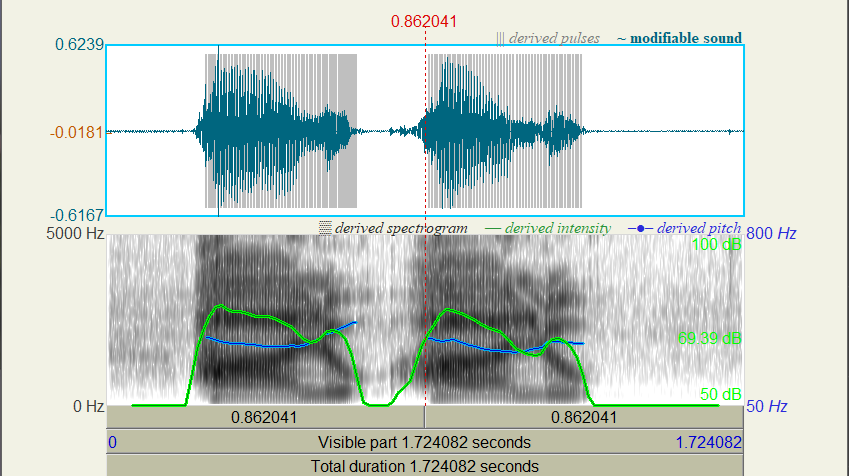
\includegraphics[width=0.65\linewidth]{img/hal_u.png}
		\caption{Reduplication of /\textipa{hal'u}/}\label{fig:hal'u}
	\end{figure}
	
	We also see the differences between the /\textipa{u}/ and the /\textipa{o}/
	sound in the spectrogram as /\textipa{u}/ tends to have a lower frequency than
	/\textipa{o}/.
	
	\begin{figure}
		\centering
		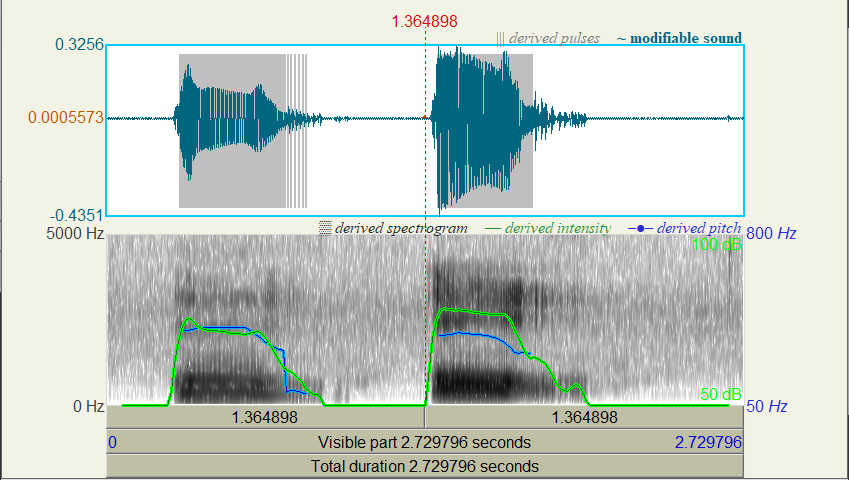
\includegraphics[width=0.65\linewidth]{img/u-o.png}
		\caption{Spectrogram of the /\textipa{u}/ and /\textipa{o}/ vowel sounds}\label{fig:u-o}
	\end{figure}
	
	It should be noted that the samples in
	\cref{fig:halo,fig:hal'o,fig:halu,fig:hal'u} do not account for potential
	allophonic changes in the syllable ``ha'' in the word ``Halo-Halo''. Here, we
	simply assume that ``ha'' is pronounced identically in both duplications.
	
	However,~\cite{KWF2015} indicates that ``Halo-Halo'' can be pronounced as
	/\textipa{h'alo hal'o}/, with a glottal stop occurring between the glottal
	fricative /\textipa{h}/ and the open front unrounded vowel /\textipa{a}/.
	\Cref{fig:a-a'} illustrates both sounds in the spectrogram.
	
	\begin{figure}
		\centering
		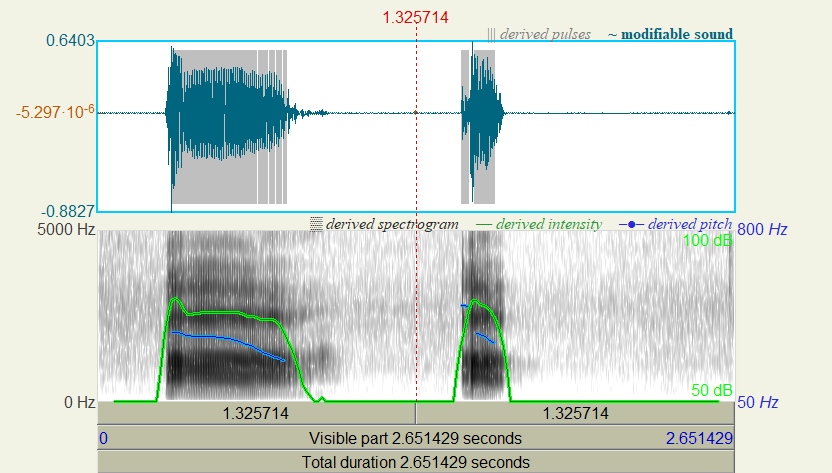
\includegraphics[width=0.65\linewidth]{img/a-a_.png}
		\caption{Spectrogram of the /\textipa{a}/ and /\textipa{'a}/ sounds}\label{fig:a-a'}
	\end{figure}
	
	The left spectrogram is the /\textipa{a}/ sound which we see is a continuous
	sound that is slowly tapering off. While, the right is the /\textipa{'a}/ sound
	which has an abrupt stop.
	
	\subsection{Correct Pronunciation of ``Halo-Halo''}
	Overall, we expect the spectrogram of ``Halo-Halo'' to display four distinct
	phonetic sections. The first section ends abruptly due to a glottal stop. It is
	followed by two syllables containing plain vowel sounds, and the final section
	ends with a vowel accompanied by another glottal stop.
	
	This pattern is observed in \cref{fig:correct}.
	
	\begin{figure}
		\centering
		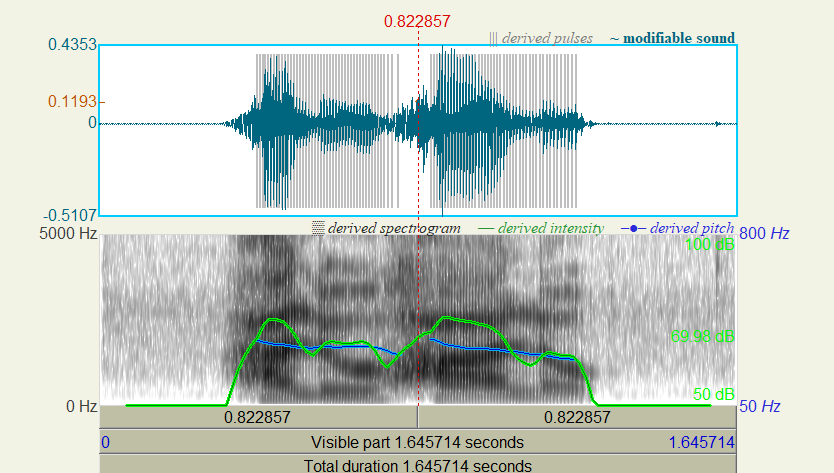
\includegraphics[width=0.65\linewidth]{img/correct.png}
		\caption{Spectrogram of the correct pronunciation of ``Halo-Halo''}\label{fig:correct}
	\end{figure}
	
	\subsection{Phonological Analysis of Mispronunciations}
	
	The observed mispronunciations of ``Halo-Halo'' can be explained in terms of
	\emph{first language (L1) interference}, particularly the influence of English
	orthography and phonotactics on non-Tagalog speakers~\cite{hansenedwards2008phonology}. English readers, when
	encountering the sequence ``halo,'' often default to pronouncing the final
	\emph{``o''} as /\textipa{u}/ rather than /\textipa{o}/. This reflects the
	English tendency to interpret word-final ``o'' as a high back rounded vowel,
	rather than the mid-back rounded vowel found in Tagalog.
	
	Additionally, the absence of explicit diacritics in common spelling
	encourages English speakers to treat ``Halo-Halo'' as a compound word with
	English stress placement, leading to flattened intonation and the omission of
	Tagalog glottal stops. The result is a pronunciation closer to
	/\textipa{halu-halu}/, which is orthographically consistent with English but
	phonologically inconsistent with Tagalog norms.
	
	\subsection{Conclusion}
	
	Variations in possible pronunciations of ``Halo-Halo'' arise from the
	widespread use of \emph{common spelling} (writing without diacritics) in most
	Philippine contexts. The word's pronunciation can be clearly inferred when
	using its \emph{diacritic orthography}: ``h\'alo-Hal\`o'', which indicates the
	stressed syllables and glottal stops.
	
	\section{Audio Characteristics of Emotion Speech}
	
	We recorded the phrase ``Your power is mine'' with the following voice actor
	profile:
	
	\begin{enumerate}
		\item \textbf{Actor:} Clarence Ang
		\item \textbf{Sex:} Male
		\item \textbf{Age range:} Adult (25--40)
		\item \textbf{Language:} English
		\item \textbf{Accent:} Philippine English
		\item \textbf{Speaking style:} Read speech with controlled emotional expressions
		\item \textbf{Emotion set:} Happy, Sad, Fear, Anger\footnote{One recording was produced for each emotion.}
		\item \textbf{Audio format:} Mono channel recordings
	\end{enumerate}
	
	The prosodic analysis of each emotional speech recording was conducted using
	Praat. The characteristics of pitch and intensity for each emotion are
	summarized in~\cref{tab:intensity,tab:pitch}:
	
	\begin{table}[h]
		\centering
		\caption{Pitch characteristics of emotional recordings}
		\begin{tabular}{ll}
			\hline
			\textbf{Emotion} & \textbf{Pitch}                                      \\
			\hline
			Happy            & Relatively stable throughout the audio              \\
			Sad              & Relatively stable, with a much lower range          \\
			Anger            & Higher pitch compared to the other emotions         \\
			Fear             & Fluctuates (drops and rises) due to vocal shakiness \\
			\hline
		\end{tabular}\label{tab:pitch}
	\end{table}
	
	\begin{table}[h]
		\centering
		\caption{Intensity characteristics of emotional recordings}
		\begin{tabular}{ll}
			\hline
			\textbf{Emotion} & \textbf{Intensity}                               \\
			\hline
			Happy            & Can rise to high levels, then drop swiftly again \\
			Sad              & Generally low, with occasional slight increases  \\
			Anger            & Spikes sharply in waves, reaching high levels    \\
			Fear             & Unstable, rising and falling with uncertainty    \\
			\hline
		\end{tabular}\label{tab:intensity}
	\end{table}
	
	\subsection{Conclusion}
	The emotional recordings exhibited distinct prosodic characteristics in terms
	of pitch and intensity. For happy speech, the pitch remained relatively stable
	while the intensity rose to high levels and dropped swiftly, reflecting
	energetic expressiveness. Sad speech showed a much lower pitch range with
	generally subdued intensity, though slight increases were observed at certain
	points. In the case of anger, the pitch was markedly higher compared to the
	other emotions, and the intensity spiked sharply in wave-like patterns,
	producing a forceful delivery. Finally, fearful speech was characterized by
	pitch fluctuations—dropping and rising due to vocal shakiness—while the
	intensity was unstable, alternating between increases and decreases that
	conveyed uncertainty.
	
	\bibliography{refs}
	\bibliographystyle{alpha}
	
	\vfill
	{\footnotesize
		\noindent\textbf{Declaration of AI Use:} The author used ChatGPT-5 to 
		assist with language editing and improving the clarity of the manuscript. 
		All content generated by the AI was carefully reviewed and edited by the 
		authors. The authors take full responsibility for the accuracy and integrity 
		of the final manuscript.
		\par}
\end{document}